\section{Resultados y análisis}

Los resultados de cada ruta se presentan en dos partes: primero se realiza una descripción geográfica de la ruta trazada, basada en las ips seguidas, prestando particular atención a los saltos intercontinentales; en la segunda parte se analizan los RTTs entre saltos, de los cuales se busca poder inferir en forma automática los enlaces intercontinentales detectados en la primer parte.

\subsection*{Universidad de São Paulo}

\subsubsection*{Recorrido en el Planisferio}

A continuación se puede ver el recorrido realizado por los paquetes enviados al destino. Como era de esperarse no se realizan saltos intercontinentales, si no que se forma un camino bastante directo de Buenos Aires a São Paulo.

De los 13 saltos necesarios para llegar al destino, 4 no respondieron el TTL, resultando en un 30\% de saltos sin respuesta de \emph{time exceeded} y un largo de ruta de 9 hops que si respondieron.

\begin{figure}[H]
  \centering
  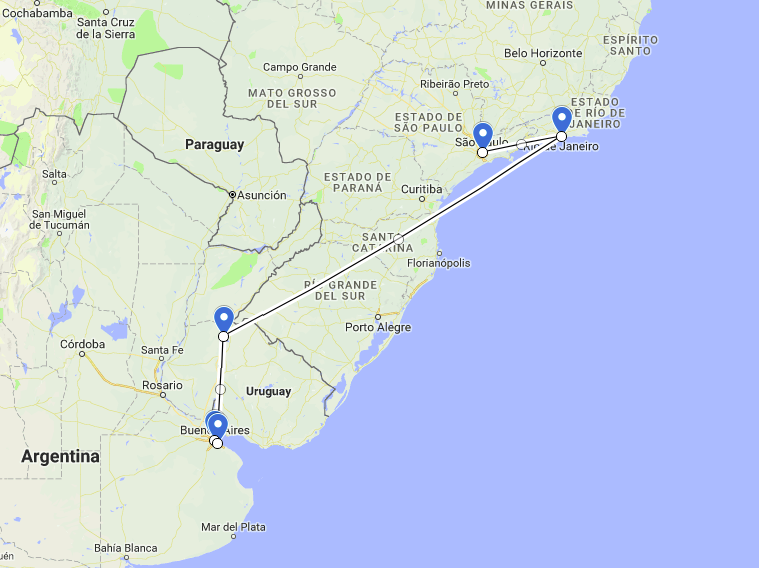
\includegraphics[width=8.5cm]{figs/saopaulo.png}
  \caption{\footnotesize Recorrido realizado por los paquetes durante la ejecución de traceroute al intentar alcanzar el sitio \texttt{www5.usp.br}}
\end{figure}

\subsubsection*{RTT entre saltos}

Analicemos cómo funciona nuestro modelo para inferir saltos intercontinentales, en un caso donde sabemos que no hay ninguno.

\begin{figure}[H]
  \centering
  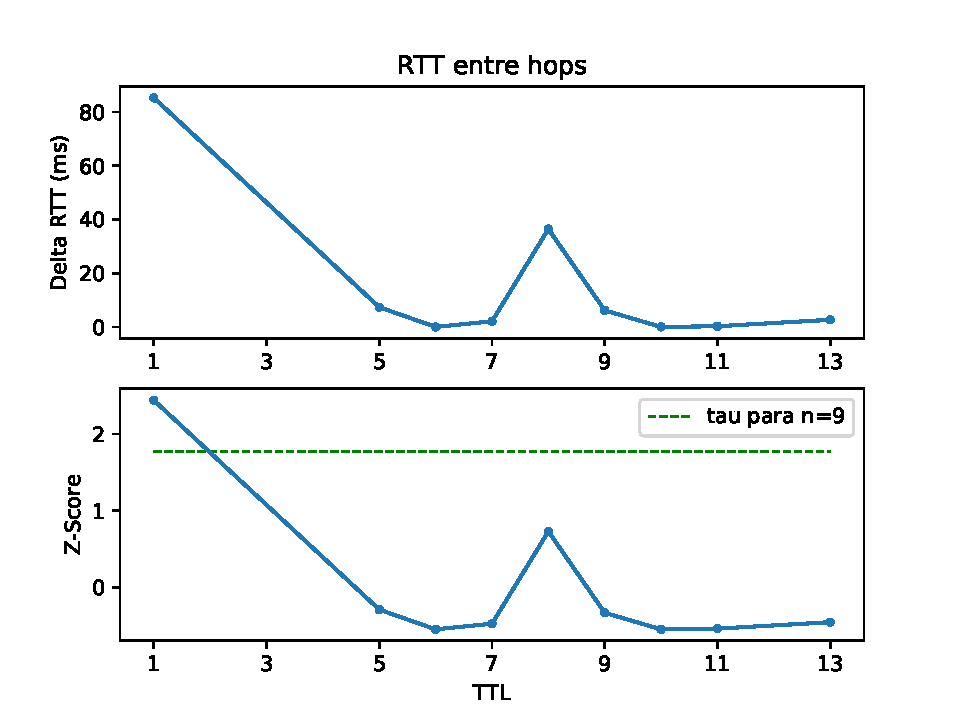
\includegraphics[width=8.5cm]{figs/traceroute-saopaulo.pdf}
  \caption{\footnotesize RTT entre saltos (antes y después de normalizar respectivamente) para el sitio \texttt{www5.usp.br}. $n$ es la cantidad de TTLs para los que se obtuvo un \emph{time exceeded} (que son los puntos que se grafican).}
  \label{plot-saopaulo}
\end{figure}

Viendo la figura \ref{plot-saopaulo}, observamos que hay un falso positivo: el RTT estandarizado del primer hop supera el umbral dado por la $\tau$ del Test de Thompson. Podemos entender esto como una consecuencia de que el test utilizado no hace más que buscar valores atípicos (en nuestro caso atípicamente grandes) dentro de una muestra. Por lo tanto, en la medida que los RTTs entre hops no sean equitativos, no es de sorprender que casi siempre encontremos algún salto que sobresalga del resto. La clave está en que si tuviéramos un trayecto significativamente más largo, este valor que ahora resulta un outlier muy posiblemente quedaría opacado por el RTT diferencial de un verdadero salto continental.

Vale decir que en este caso particular, lo que parece estar sucediendo es que hay una cuestión técnica de la LAN desde la cual se dispara el \emph{traceroute} que dificulta alcanzar el \emph{gateway}, pues 80ms parece un tiempo elevado para esto. Independientemente, se probó llegar al mismo destino desde otra LAN con mejor tiempo de llegada al \emph{gateway}, y sin embargo también se obtuvo un outlier en un hop posterior, reafirmando el punto anterior de que lo que se considera un outlier depende fuertemente de la escala de la ruta. 

\subsection*{Universidad de Moscú}

\subsubsection*{Recorrido en el Planisferio}

A continuación se puede ver el recorrido realizado por los paquetes enviados al destino, este en principio puede ser extraño ya que realiza 3 saltos intercontinentales, en vez de 1 o 2 como era de esperarse, más adelante nos explayaremos un poco sobre las razones por las cuales pudo haber sucedido esto.

De los 30 saltos necesarios para llegar al destino 3 no respondieron el TTL, resultando en un 10\% de saltos sin respuesta de time exceeded y un largo de ruta de 27 hops que si respondieron.

\begin{figure}[H]
  \centering
  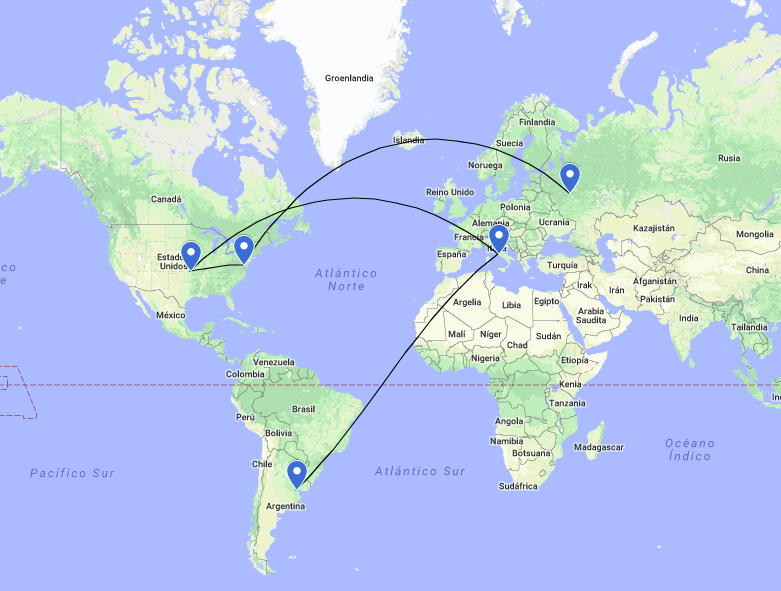
\includegraphics[width=8.5cm]{figs/moscow.png}
  \caption{\footnotesize Recorrido realizado por los paquetes durante la ejecución de traceroute al intentar alcanzar el sitio \texttt{www.msu.com}}
\end{figure}

\subsubsection*{RTT entre saltos}

\begin{figure}[H]
  \centering
  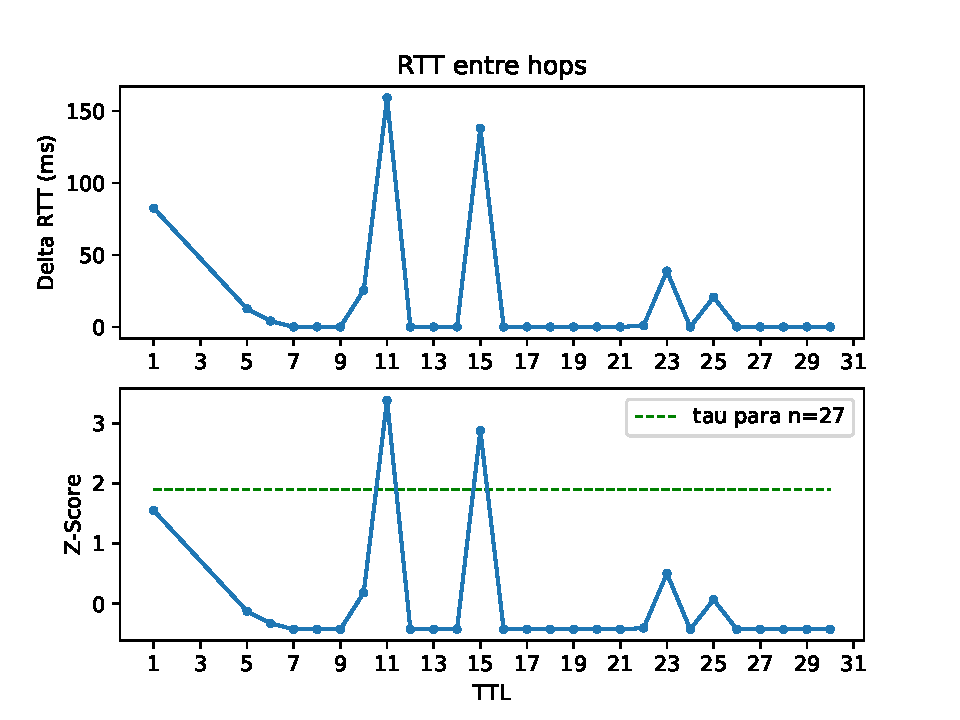
\includegraphics[width=8.5cm]{figs/traceroute-moscow.pdf}
  \caption{\footnotesize RTT entre saltos (antes y después de normalizar respectivamente) para el sitio \texttt{www.msu.com}. $n$ es la cantidad de TTLs para los que se obtuvo un \emph{time exceeded} (que son los puntos que se grafican).}
  \label{plot-moscow}
\end{figure}

Para este caso, podemos observar en la figura \ref{plot-moscow}, que se detectan dos saltos intercontinentales. Este caso tiene bastantes particularidades, relacionadas con la ruta compleja que se vió en el punto anterior. 

El primer pico, que se da en el salto 11, coincide con un salto a un router de Roma, Italia (\texttt{89.221.41.171}). La cuestión es que el nodo desde el cual se realiza el hop también está ubicado en Italia (\texttt{185.70.203.32}), y dicho salto no fue detectado como outlier, pues en efecto tiene un RTT mucho más bajo. Una posible hipótesis que manejamos al respecto de porqué ocurrió esto (que no se detecte el salto continental, pero sí el siguiente hop) es que el primer router al que se llega sea uno de los principales gateways de Italia, lo que provoque que se encuentre congestionado y el paquete que se manda quede encolado un largo tiempo antes de forwardearse al siguiente hop. 

El segundo pico, con TTL 15, presenta una situación similar: el destino está en Estados Unidos, pero los tres saltos anteriores también, y no fueron detectados. Acá hay una diferencia sin embargo: esos tres saltos mostraron todos RTTs diferenciales de 0, lo que implica que de hecho el RTT promedio de estos nodos fue menor que el promedio del último router que estaba en Italia. Este parece ser un caso de \textit{camino asimétrico} (Jobst 2012). Razonablemente existe una mejor ruta desde Estados Unidos a Argentina, que cruzar toda Europa. Que la ruta no haya ido directamente por Estados Unidos, salteandose Italia, suena a una consecuencia de un cambio del estado de la red: posiblemente el paquete se mandó a Italia porque había una ruta aprendida que iba directamente de Italia a Rusia sin salir del continente, pero por alguna razón dicho camino \emph{óptimo} dejó de estar habilitado.

En definitiva, hay que decir que en este caso tuvimos dos falsos positivos y tres falsos negativos (Argentina-Italia, Italia-USA, USA-Rusia). 

Algo para señalar, es que este caso se corrió desde la misma LAN que la ruta anterior, y puede verse en los gráficos que efectivamente el RTT del primer salto fue igual, pero en este caso, a diferencia del anterior, no se consideró un \emph{outlier}, pues había saltos mucho más costosos. Esto viene a fortalecer la hipótesis de que la longitud de la ruta afecta la calidad de la inferencia.

\subsection*{Universidad de Sidney}

\subsubsection*{Recorrido en el Planisferio}


A continuación se puede ver el recorrido realizado por los paquetes enviados a Sidney, se realizaron 2 saltos intercontinentales. Uno de Argentina a Estados Unidos y otro de Estados Unidos a Australia lo cual parece indicar que no hay una conexión directa de América del Sur a oceanía pero si desde América del Norte.

De los 26 saltos necesarios para llegar al destino 6 no respondieron el TTL, resultando en un 23\% de saltos sin respuesta de time exceeded y un largo de ruta de 20 hops que sí respondieron.

\begin{figure}[H]
  \centering
  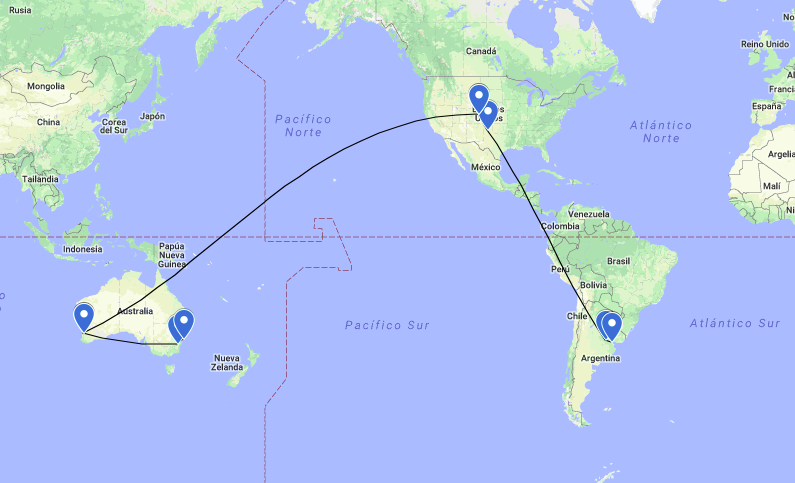
\includegraphics[width=8.5cm]{figs/sidney.png}
  \caption{\footnotesize Recorrido realizado por los paquetes durante la ejecución de traceroute al intentar alcanzar el sitio \texttt{sydney.edu.au}}
\end{figure}

\subsubsection*{RTT entre saltos}

\begin{figure}[H]
  \centering
  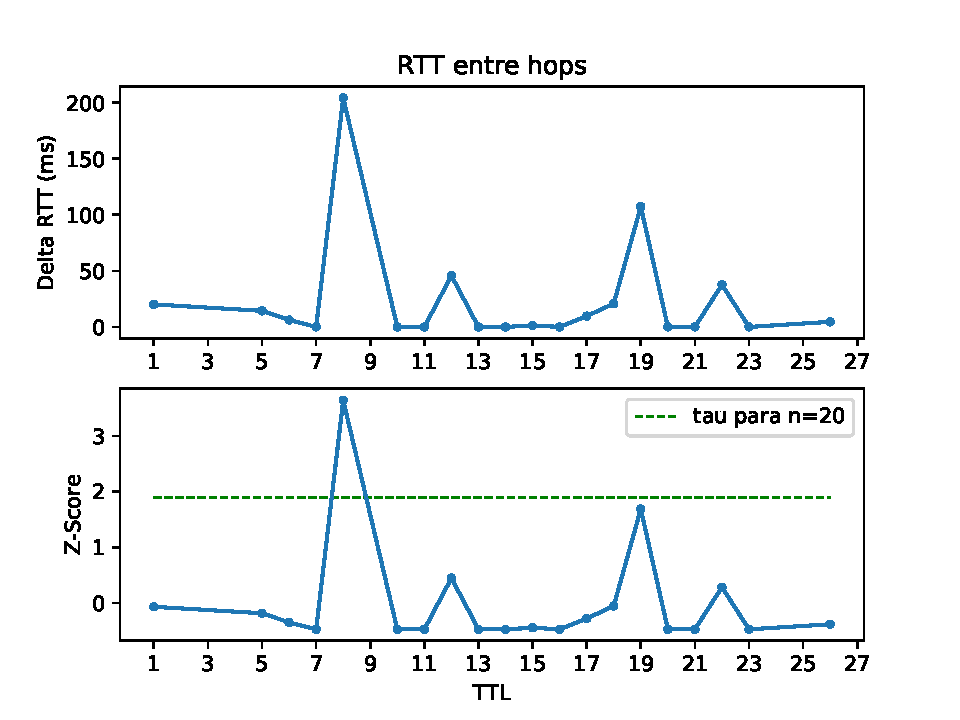
\includegraphics[width=8.5cm]{figs/traceroute-sidney.pdf}
  \caption{\footnotesize RTT entre saltos (antes y después de normalizar respectivamente) para el sitio \texttt{sydney.edu.au}. $n$ es la cantidad de TTLs para los que se obtuvo un \emph{time exceeded} (que son los puntos que se grafican).}
\end{figure}

Finalmente, para esta ruta vemos que se detectó un salto intercontinental en el octavo hop. Este efectivamente fue un salto de Argentina a Estados Unidos (que como mencionamos en la sección anterior, vamos a considerar un salto continental). Por otro lado, no se detectó el salto de Estados Unidos a Australia en el salto 19, aunque puede verse en el gráfico que estuvo bastante cerca de alcanzar el threshold.

Para esta ruta tuvimos entonces un falso negativo, y un verdadero positivo.

Algo que puede valer la pena mencionar de este caso es que la mayoría de los valles donde el delta RTT da 0ms son saltos donde la diferencia de tiempo es menor que la varianza, lo cual es razonable ya que se mueven entre nodos que están cercanos entre sí.
